
\subsection{Textual Analysis}


We examine syntactic and semantic properties 
of the highlighted text so that 
we might identify
common cues to the relevancy of text to a task (\textit{RQ2}).
Since we intend to use these cues 
in the design of a general technique, 
we examine the text across 
all the kinds of artifacts 
available for all the tasks. 




 
% For instance, consider the sentence:
% ``\textit{you can use include\_fields if you want specific field names}''.
% We can extract the elements dependent upon the the verb `\textit{use}' (i.e., {\small \texttt{[nsubject, use, code\_word]}})
% and, if we observe that these elements co-occur in multiple HUs, we flag the pattern as a cue to the relevancy of the text.





\subsubsection{Does syntactic structure provide cues to the relevancy of text to a task?}
\label{cp3:syntactic-analysis}


For our syntactic analysis, we follow procedures from related work (Section~\ref{cp2:nlp}).
We start by inspecting the elements that compose a sentence (i.e., nouns and verbs)
and then, we analyze possible patterns that may arise from the syntactic structure of the text~\cite{Robillard2015},
investigating if the extracted entities co-occur in multiple HUs.



% We start our syntactic analysis by describing noun phrases and verb phrases
% in the relevant text. 
% We then describe our analysis of syntactic patterns.  



Among noun phrases, we observe that 65\% of the HUs contain acronyms or coding elements.
Existing approaches that rely on these elements to identify relevant text (e.g.,~\cite{Robillard2015} or~\cite{Jiang2016b}) would miss the remaining 35\% of the HUs in our corpus.
This value may seem acceptable at first; however, there are no guarantees that
the identified 65\% HUs hold all the crucial information for task completion.
As an example, some of the HUs from the mid and topmost tiers 
do not contain obvious code elements that could signal their relevancy,
such as one of the sentences in the \texttt{Bugzilla} task that indicates the need for ``\textit{authentication to allow retrieving non-public data}''.
% The lack of authentication implies missing non-public data, which leads to an incomplete solution, 
% and so this sentence was considered relevant by most of the participants in our study
% even when it .





With regards to verb phrases, we observe a substantial
overlap (81\%) with verbs observed in Ko and colleagues linguistic analysis
of bug report titles~\cite{Ko2006}.
The most common verbs in the HUs include conjugations of verbs such as \textit{use}, \textit{get}, \textit{set}, \textit{be}, or \textit{do},
but with the exception of \textit{use}, \textit{get}, and \textit{set}, the
remaining top common verbs are in English stop words lists~\cite{jurafsky2014speech}. As a result, many
\acs{NLP} techniques would discard them as part of their pre-processing
steps~\cite{Bavota2016}.






As for syntactic patterns, we did not observe a large set of patterns for the variety of tasks and artifacts in our experiment,
where the prominent patterns identified (e.g., $\{$\textit{nsubject, do, negation}$\}$)
reflect common constructs of the English language rather than cues that we might explore for the relevancy of text.
There may be multiple explanations for these results, such as
the fact our corpus contains a small number of natural language artifacts.
Due to this reason, we also checked whether patterns from existing related work (i.e.,~\cite{Chaparro2017, Robillard2015}) applied to the text in our HUs, 
but the small number of matching patterns 
raises caution on
their generalizability.



\medskip
\begin{bluequote}
    \textit{We did not find prominent syntactic cues to identify
    task-relevant information. Our analysis of highlights demonstrates:
    1) limitations of existing techniques that rely on code
    elements and acronyms, 2) missed
    information that may occur due to the prevalence of verbs that
    appear in English stop word lists,
    and 3) the absence of patterns derived from the syntactic structure of
    the text.}
\end{bluequote}

 



\subsubsection{Do semantics provide cues to the relevancy of text to a task?}
\label{cp3:semantic-analysis}


For our semantic analysis, we
analyze the meaning of the text in the 
 HUs
using frame semantic parsing~\cite{fillmore1976frame, jurafsky2014speech}.
Semantic frames are centered around events, called \textit{frames}, 
which abstract both the event
as well as relationships, entities or participants related to that
event~\cite{fillmore1976frame, Baker1998}. 


We explain semantic frames by considering
 two distinct sentences extracted 
from the \texttt{Databases} and the \texttt{Lucence} tasks, respectively.
For each sentence, Figure~\ref{fig:frame-examples} shows an
excerpt of the frame analysis for the sentences. 
The frames of each sentence (in grey) represent a triggering event and the frame elements \textit{(fe)} (in red) are arguments needed to understand the event. The enclosing square brackets mark all lexical units, or words, associated with either a frame or a frame element.
Observing the frame elements captured by the verbs `\textit{see}' and
`\textit{understand}', both sentences have the common meaning of
describing a `\textit{phenomenon}'.
However, the frame elements
that capture the meaning of each verb differ: the former represents a
`\textit{perception of experience}' while the latter represents a
cognizer `\textit{grasp}'ing her knowledge over the 
phenomenon. 





% \begin{figure}[h!]
% \fbox{%
% \parbox{0.49\textwidth}{%
% }}
% \label{sec:frames-lucene}
% \end{figure}


\begin{figure}
\begin{mdframed}
\begin{scriptsize}
\noindent \textbf{Databases:} \textit{I have yet to see a situation where hibernate was the reason for poor performance in production.}
{\ttfamily% 
\begin{enumerate}[itemindent=0.5em,leftmargin=0.5em]
\item[] $\big[$I$\big]$\textsubscript{\color{rufous} \textbf{fe:perceiver}} have yet to $\big[$see$\big]$\textsubscript{\hl{\textbf{perception of experience}}} 

\item[] $\big[$a situation where hibernate was the reason for \dots$\big]$\textsubscript{\color{rufous} \textbf{fe:phenomenon}}
\end{enumerate}
}%

\smallskip
\noindent \textbf{Lucence:} \textit{As far as I understand that sums up totalTermFreqs for all terms of a field}
{\ttfamily% 
\begin{enumerate}[itemindent=0.5em,leftmargin=0.5em]
\item[] As far as $\big[$I$\big]$\textsubscript{\color{rufous} \textbf{fe:cognizer}} $\big[$understand$\big]$\textsubscript{\hl{\textbf{grasp}}} 

\item[] $\big[$that sums up totalTermFreqs for all terms of a field$\big]$\textsubscript{\color{rufous} \textbf{fe:phenomenon}}
\end{enumerate}
}%
\end{scriptsize}
\end{mdframed}
    \caption{Example of frames and frame elements}
    \label{fig:frame-examples}
\end{figure}

As multiple sentences might have similar meanings,
we analyze whether there are common frame elements 
that provide cues to the relevancy of text.
For this analysis, all frame elements were extracted automatically
using the \textit{SEMAFOR} tool~\cite{das2014frame},
where we extract the frames of every HU, resulting in 3,719 frames across
the 602 HUs. Only 346 distinct frames appear across these 3,719 frames
parsed. The proportionally small number of distinct semantic frames
occurring suggests that different HUs share frame elements
and thus, we further inspect the most common frames identified.



Table~\ref{tbl:common-frames} details the most frequent frames identified per tier, filtering to show the 
most frequent frames in a tier that have not appeared in lower tiers.
In the top-most tier, the most frequently identifying distinguishing
frames denote the `\textit{cause}' or `\textit{likelihood}' of a phenomenon.
These frames are found in sentences that explain a system's behavior, which are often crucial for task completion,
as in a sentence that provides a cause for the loss in performance when using Hibernate:
 \textit{``if you need to process lots of objects for some reason, though it can seriously affect performance}''.
Other common frames \textit{quantify relationships},
as when a sentence describes the minimum elements needed to perform an operation, e.g., \textit{``to create a flag, at least the status and the type\_id or name must be provided}''.


\afterpage{


\begin{landscape}


\begin{table}
\caption{Most common semantic meanings across all the HUs; frames are presented per tier, from the topmost tier to the bottom tier} 
\begin{scriptsize}
\vspace{-1mm}  
\begin{threeparttable}    
\begin{tabular}{|l|lclr|}

\cline{2-5}       
% 
\multicolumn{1}{c|}{} &
\textbf{Frame} &
\textbf{Freq} &
\textbf{Description} & 
\parbox[l][.4cm][c]{9.8cm}{\textbf{Example}}

\\ \hline

&
\cellcolor{lightgray} Likelihood &
\cellcolor{lightgray} 8\% & 
\parbox[l][1.2cm][c]{4.4cm}{\cellcolor{lightgray} Denotes the likelihood of a hypothetical event occurring}  &
\parbox[l][1.2cm][c]{9.8cm}{\cellcolor{lightgray} \texttt{However, it can be overkill for some types of application, and the backend \underline{could be easier} to implement with a protocol such as SSE.}} \\

\multirow{-2}{*}{\rotatebox[origin=l]{90}{\textbf{top tier}}} &
Causation &
8\% & 
\parbox[l][.8cm][c]{4.4cm}{An effect is observable due to a cause} &
\parbox[l][.8cm][c]{9.8cm}{\texttt{By default this is true, \underline{meaning} overlap tokens do not count when computing norms. }} \\

&
\parbox[l][.8cm][c]{1cm}{\cellcolor{lightgray} Relational \\ Quantity} &
\cellcolor{lightgray} 7\% & 
\parbox[l][.8cm][c]{4.4cm}{\cellcolor{lightgray} Denotes a quantifiable relationship between any two dependent entities}  &
\parbox[l][.8cm][c]{9.8cm}{\cellcolor{lightgray} \texttt{It is \underline{much faster} to get to something working with Hibernate \underline{than it is} with JDBC }} \\

\hline
\hline

&
\parbox[l][.8cm][c]{1cm}{Statement} &
12\% & 
\parbox[l][.8cm][c]{4.4cm}{Verbs and nouns that communicate the act of a speaker to address a message } &
\parbox[l][.8cm][c]{9.8cm}{\texttt{Custom fields \underline{are} normally returned by default unless this is added to exclude\_fields }} \\

\multirow{3}{*}{\rotatebox[origin=l]{90}{\textbf{mid tier}}} &
\parbox[l][.8cm][c]{1cm}{\cellcolor{lightgray} Intentionally \\ act} &
\cellcolor{lightgray} 11\% & 
\parbox[l][.8cm][c]{4.4cm}{\cellcolor{lightgray} An act performed by an entity} &
\parbox[l][.8cm][c]{9.8cm}{\cellcolor{lightgray} \texttt{The data field could, of course, have any string data; \underline{it doesn't have to be} JSON. }} \\

&
\parbox[l][.8cm][c]{1cm}{Fields\tnote{\dag}} &
11\% & 
\parbox[l][.8cm][c]{4.4cm}{Denotes mentioning an object attribute or field} &
\parbox[l][.8cm][c]{9.8cm}{\texttt{computeNorm(FieldInvert state) - computes the normalization value
for a \underline{field} }} \\

&
\parbox[l][.8cm][c]{1cm}{\cellcolor{lightgray} Being \\ returned\tnote{\dag}} &
\cellcolor{lightgray} 11\% & 
\parbox[l][.8cm][c]{4.4cm}{\cellcolor{lightgray} Denotes results from a particular operation or method call} &
\parbox[l][.8cm][c]{9.8cm}{\cellcolor{lightgray} \texttt{You need to be aware of this behaviour otherwise \underline{you will get} cryptic errors}} \\

\hline
\hline

\multirow{3}{*}{\rotatebox[origin=r]{90}{\textbf{bottom tier}}} &
Using &
17\% & 
\parbox[l][.8cm][c]{4.4cm}{An agent uses an instrument in order to achieve a purpose} &
\parbox[l][.8cm][c]{9.8cm}{\texttt{By \underline{using JDBC}, resource leaks and data inconsistency happens as work is done by the developer.}} \\

&
\cellcolor{lightgray} Purpose &
\cellcolor{lightgray} 15\% & 
\parbox[l][.8cm][c]{4.4cm}{\cellcolor{lightgray} Denotes a goal or target to be achieved} & 
\parbox[l][.8cm][c]{9.8cm}{\cellcolor{lightgray} \texttt{Object Relational Mapping \underline{empowers the use of} ``Rich Domain Object'' which are Java classes}} \\

&
Capability & 
14\%  & 
\parbox[l][.8cm][c]{4.4cm}{An entity does or does not meet the pre-conditions for some event or action} & 
\parbox[l][.8cm][c]{9.8cm}{\texttt{\underline{Can't} detect anything outside letters, arrows, ctrl, alt and shift}} \\

\hline

\end{tabular}
\begin{tablenotes}
    \item[\dag] \scriptsize Frame name was modified because its semantic meaning is specific to software engineering;    
\end{tablenotes}
\end{threeparttable}    
\end{scriptsize}
\label{tbl:common-frames}
\end{table}
\end{landscape}
}


In the middle tier, we observe frames for actions performed by some entity (\textit{intentionally act}) or facts regarding a topic (\textit{statement}).
Other common frames relate to methods or attributes and the result of some operation such as a method call, which may be useful for identifying code related entities.
For instance, this sentence from the \texttt{Bugzilla} tasks contains both the `\textit{being returned}' and the `\textit{fields}' frame, 
\textit{``You can specify to only return custom fields by specifying \_custom or the field name in include\_fields''}.



The bottom tier contains frames that are common to all HUs.
The most frequent frame in the bottom tier has a semantic meaning of `\textit{using}'.
HUs with this frame are often sentences detailing how to use a method or a
framework to achieve some goal, which might also explain the second most frequently occurring frame, i.e., `\textit{purpose}', which denotes an achievable goal. 
These two frames could be used to filter sentences that contain the means
to use a technology or API with certain intention, as in this sentence explaining usage scenarios for
WebSocket and Server-Sent Events in the \texttt{Networking} task:
``\textit{One is synchronous and could/would be used for near real-time data xfer, whereas the other is asynchronous and would serve an entirely different purpose}''.




To provide further evidence supporting these findings,
we also  compared the frequency of the frame elements identified in relevant text (i.e., HUs) and non-relevant text.
Figure~\ref{fig:frame-distribution} provides insight in the distribution of frames across relevant and non-relevant sentences.
For example, frames that represent a `\textit{required}' event
are more prominent in the relevant text
as found in a sentence that describes
how to circumvent errors in the \texttt{Bugzilla} REST API  due to invalid tokens:
``\textit{An error is thrown if you pass an invalid token; you will need to log in again to get a new token}''.
On the other hand, frames that relate to user discussions and that do not draw conclusions or provide 
facts about an API or technology, such as `\textit{point of dispute}' or `\textit{reasoning}' are often found in non-relevant text,
as when users discuss community's procedures in the \texttt{GPMDPU} task: ``\textit{Open a new issue following the template so we can have more details on your device}''. 


\begin{figure}
\centering
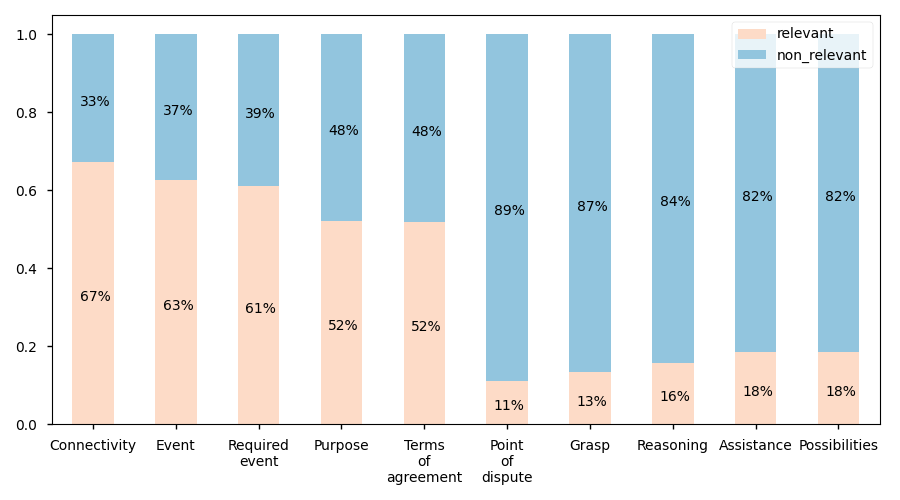
\includegraphics[width=.95\textwidth]{cp3/frames-dist-all}
\caption{Distribuion of semantic frames over the text; the figure depicts the top five frames most commonly observed in relevant and non-relevant sentences, respectively}
\label{fig:frame-distribution}
\end{figure}


\begin{figure}
\centering
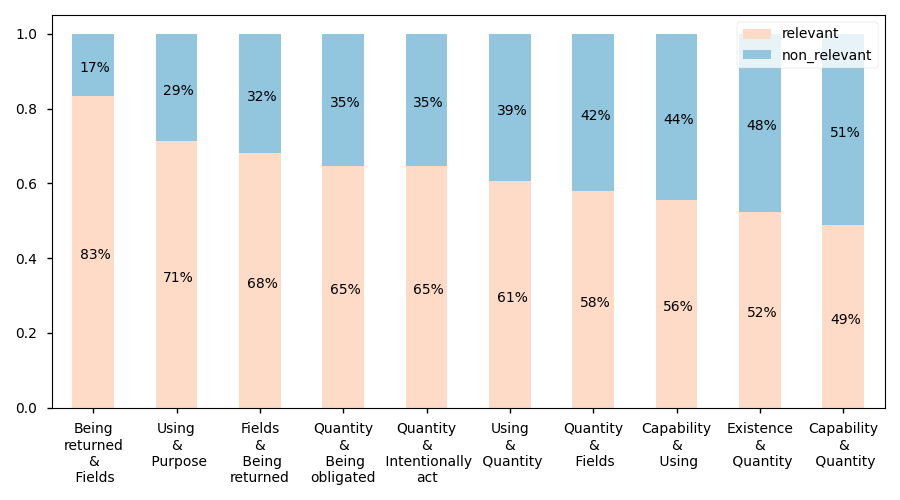
\includegraphics[width=.95\textwidth]{cp3/frames-dist-2-grams}
\caption{Distribution of co-occurring frames over the text}
\label{fig:frame-co-occurrence}
\end{figure}


While certain frames are not indicative of relevance when found on their own, we also observe that the co-occurrence of certain frames in a sentence increase the likelihood of the sentence's relevancy.
For instance, `\textit{purpose}' and `\textit{using}' occur almost evenly across relevant and non-relevant text
while their co-occurrence is more frequent in relevant text. 
Figure~\ref{fig:frame-co-occurrence} shows the most frequent frames that co-occur and their ratio on relevant and non-relevant text.


A Wilcoxon signed-rank test~\cite{wohlin2012} over the distribution of frames in our data both in individual frames and pairs of frames shows statistical significance ($p\text{-value} \le 0.05$) 
on the prominence of certain frames in relevant or non-relevant sentences.







Our analysis on the semantics of relevant text provides initial evidence that there exists some common aspect in the meaning of 
 the different sentences deemed as relevant.






\medskip
\begin{bluequote}
    \textit{There are recurring semantic meanings in relevant sentences,
    suggesting commonalities in their conveyed information
    and indicating that text might be identified through its semantics.}
\end{bluequote}



















    

